\documentclass{article}

\usepackage[utf8]{inputenc}
\usepackage[english]{babel}
\usepackage{graphicx}
\usepackage{listings}
\usepackage{xcolor}                 % Define custom colour and use using \textcolor{colour}{text}
\usepackage{float}

\usepackage{rotating}               % 90 degrees image
\usepackage{lscape}                 % landscape 

\usepackage{hyperref}

\usepackage{longtable}              % Predefined width table
\usepackage{csquotes}               % Use proper \enquote{quotations}

\usepackage[block=ragged,alldates=comp]{biblatex} % Reference management

\usepackage{tikz}
\usepackage{tikz-qtree}

\addbibresource{references.bib}

\usepackage%
[%
left=2cm,% left margin
right=2cm,% right margin
top=3cm, % top margin
bottom=3cm,% bottom margin
a4paper% other options: a0paper, a1paper, a2paper, a3paper, a4paper, a5paper, a6paper, and many more.
]{geometry}

\usepackage{pbox}

\title{DLLGraph}
\author{Youri Klaassens, Nathan Godefroij}
\date{October 2019}

\definecolor{mGreen}{rgb}{0,0.6,0}
\definecolor{mGray}{rgb}{0.5,0.5,0.5}
\definecolor{mPurple}{rgb}{0.58,0,0.82}
\definecolor{backgroundColour}{rgb}{0.95,0.95,0.92}

\setlength{\parindent}{0pt}

\lstdefinestyle{CStyle}{
    backgroundcolor=\color{backgroundColour},   
    commentstyle=\color{mGreen},
    keywordstyle=\color{magenta},
    numberstyle=\tiny\color{mGray},
    stringstyle=\color{mPurple},
    basicstyle=\footnotesize,
    breakatwhitespace=false,         
    breaklines=true,                 
    captionpos=b,                    
    keepspaces=true,                 
    numbers=left,                    
    numbersep=5pt,                  
    showspaces=false,                
    showstringspaces=false,
    showtabs=false,                  
    tabsize=2,
    language=C
}

\tikzset{every tree node/.style={minimum width=2em,draw,circle},
         blank/.style={draw=none},
         edge from parent/.style=
         {draw, edge from parent path={(\tikzparentnode) -- (\tikzchildnode)}},
         level distance=1.5cm}

\lstdefinestyle{ValgrindStyle}{
    backgroundcolor=\color{backgroundColour},   
    breakatwhitespace=false,         
    breaklines=true,                 
    captionpos=b,                    
    keepspaces=true,                 
    numbers=left,                    
    numbersep=5pt,                  
    showspaces=false,                
    showstringspaces=false,
    showtabs=false,                  
    tabsize=2,
    language=C
}

\begin{document}

\begin{titlepage}
	\centering
	\smallbreak                         % smallbreak, medbreak, bigbreak
	\rule{\linewidth}{0.2 mm} \\[0.4 cm]
	{\huge \bfseries Basic Real-Time Operating System}\\
	\smallbreak
	\par{\large targeting the ARMv7-M architecture}      
	\rule{\linewidth}{0.2 mm} \\[1.5 cm]
	\vspace*{0.5 cm}
	\par{\LARGE \textit{ROS01}, Rotterdam \today }\\[1.0 cm]
    
\includegraphics[scale=0.99]{img/HR.png}\\[1.0 cm]	

	


\begin{figure}[!b]
	\begin{minipage}{0.5\textwidth}
		\begin{flushleft} \large
			\emph{Student:}\\
		    Nick van Endhoven\\
            0998831hr.nl\\
            Breda\\
			\end{flushleft}
			\end{minipage}~
			\begin{minipage}{0.5\textwidth}
 
		\begin{flushright} \large
            \emph{Student:}\\
			Youri Klaassens\\
            0996211@hr.nl\\
            Zwaag\\
		\end{flushright}
        
	\end{minipage}\\[2 cm]
\end{figure}
    
    
    
    
	
\end{titlepage}


\tableofcontents
\thispagestyle{empty}

\newpage

\pagenumbering{arabic}
\setcounter{page}{1}

\section*{Version history}
\addcontentsline{toc}{section}{Version history}

\definecolor{darkpink}{rgb}{1.0, 0.13, 0.32}

\begin{longtable}{| p{.08\textwidth} | p{.12\textwidth} | p{.38\textwidth} | p{.30\textwidth} |}

    \hline
    \textcolor{darkpink}{Version} & \textcolor{darkpink}{Date} & \textcolor{darkpink}{Change(s)} & \textcolor{darkpink}{Note} \\
     
    \hline
    \textbf{0.1} & 11-30-2019 & Initial document & Created version history, introduction, acknowledgement and appendix. \\

    \hline

    \textbf{0.2} & 12-07-2019 & Minor changes in Appendix \ref{subsec:appendix_delay} & Documented the first assignment (toggling LEDs) \\

    \hline

    \caption{Overview of the different versions}
    \label{tab:version}

\end{longtable}


\newpage
\section{Introduction}

For the Real-time Operating Systems course (ROS01) taught at Rotterdam University of Applied Science,
the authors had to implement a scheduler for a Real-time Operating System developed by one lecturers.
Because these types of programming issues like implementing a scheduler require the programmer to be able to program at a low level and it cannot be assumed that every student following this course is familiar with low level progamming (both in the C programming language and assembler), this course contains multiple assingments to bridge this gap.
The code has been flashed and tested on the CC3220s development board (Figure \ref{fig:cc3220s}). The compiler used is TI v18.12.2.LTS.

What's worth mentioning is that some code snippets in this document make a function call to \texttt{delay\_1sec()}.
Because this is used quite a few times and redundant to have multiple definitions in this document its implementation can be seen in Appendix \ref{subsec:appendix_delay}.


\begin{figure}[H]
    \centering

    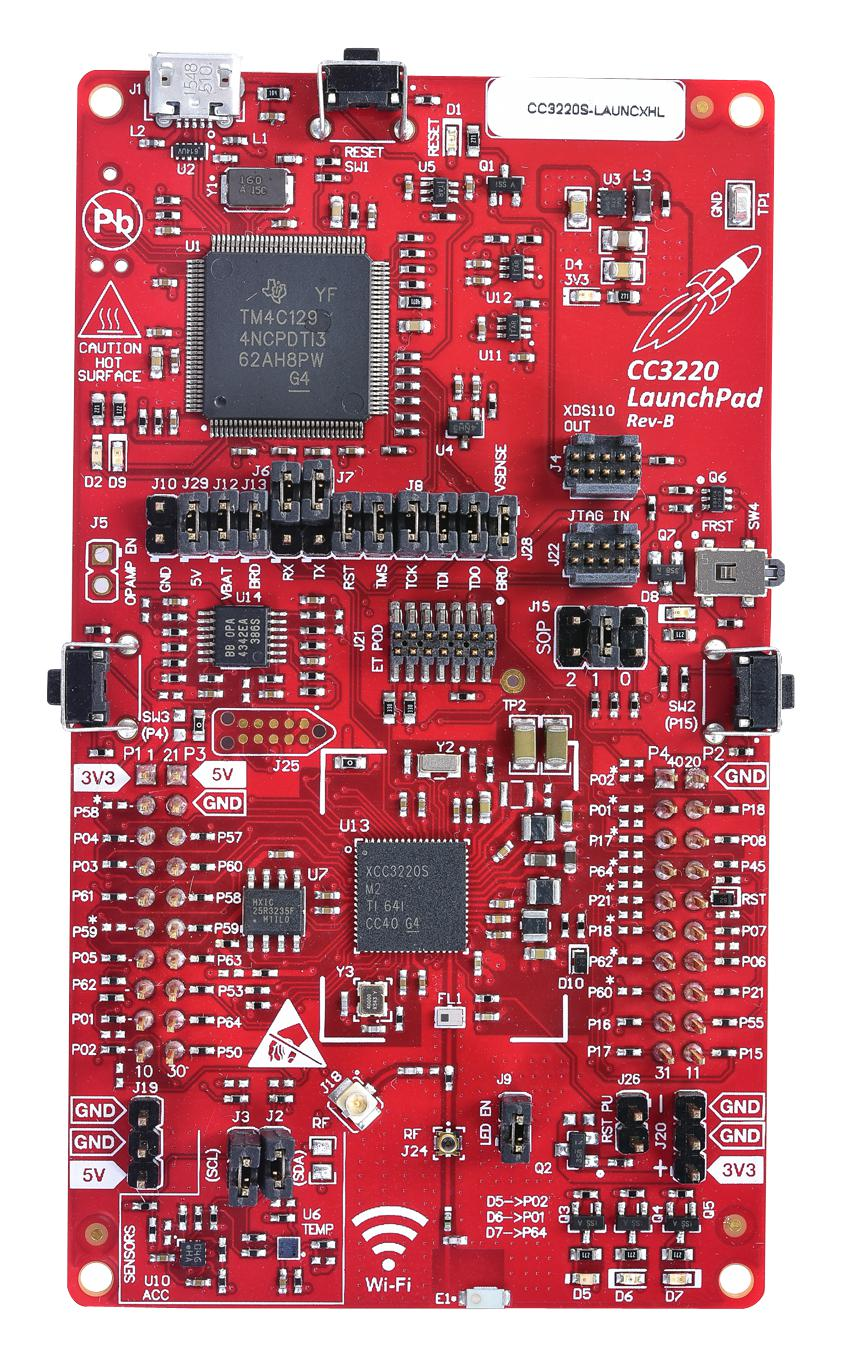
\includegraphics[angle=90,scale=0.2]{img/cc3220s.jpg}

    \caption{The CC3220s development board used during labs}
    \label{fig:cc3220s}

\end{figure}


\newpage
\section{Acknowledgement}

The authors want to thank Daniel Versluis for writing his Minimal Working Example (MWE) Real-time Operating Systems \enquote{VersdOS} and providing the authors access to the source code.
The authors also want to thank Harry Broeders for his time and effort in solving the problem related to the \texttt{delay\_1sec()} function and inline assembly instruction cycles mismatch.


\newpage
\appendix
\section{Appendix}

The appendix contains subsections that support this report or its where its content goes too much off-topic with the purpose of 
this report, but are interesting for the reader to possibly read.

\subsection{Delay \textit{exactly} one second counting instruction cycles}
\label{subsec:appendix_delay}

Many assignments require a delay of 1 second to spot blinky LEDs by eye.
One can use the Systick timer or hardware timers, but where is the fun in that?
For the sake of some assignments, it is acceptable to burn clock cycles by wasting the CPU.
Listing \ref{lst:delay1sec} contains a function which will delay the return moment by 1 second.
Now each line containing inline assembly will be explained.

\begin{lstlisting}[style=CStyle, caption={C function containing inline assembly to perform a delay of \textit{exactly} one second}, captionpos=b, label={lst:delay1sec}, escapechar=|]
void delay_1sec(void)
{
    __asm("    PUSH {r4-r11,lr}");  |\label{line:delay1sec_push}|
 
    __asm("    LDR r4, [pc, #12]"); |\label{line:delay1sec_getword}|
   
    __asm("    MOV r5, pc");        |\label{line:delay1sec_storepc}|
    __asm("    NOP");               |\label{line:delay1sec_nop}|
     
    __asm("    SUBS r4, #1");   /* 1 instruction cycle */ |\label{line:delay1sec_sub}|
    __asm("    ITE NEQ");       /* 1 instruction cycle */ |\label{line:delay1sec_ite}|
   
    __asm("    MOV pc, r5");    /* 1 + P instructions (where P is between 1 and 3 depending on pipeline refill) */ |\label{line:delay1sec_restorepc}|
     
     
    __asm("    POP {r4-r11,pc}"); |\label{line:delay1sec_pop}|
    __asm("    .word    0x5000000"); |\label{line:delay1sec_word}|
}
\end{lstlisting}

Line \ref{line:delay1sec_push} pushes 8 registers onto the stack. 
This is part of the ARM Architecture Procedure Call Standard (AAPCS) which is part of the ARM Application Binary Interface (ABI) \cite{IntroEmbeddedSystems}.
This standard describes that \texttt{R0} up to and including \texttt{R4} are used to pass input parameters into a C function. 
Functions should preserve the content of registers \texttt{R4} up to and including \texttt{R11}.
Listing \ref{lst:delay1sec} does not use all of the registers a callee should save, but it is best practice to push them in case one does not know how many registers his or her piece of software will use.\\
%TODO: Explain line two
Line \ref{line:delay1sec_storepc} stores the Program Counter (PC) into \texttt{R5}. 
Because the PC is two instruction (8 bytes) ahead in ARM mode it actually stores the address for Line \ref{line:delay1sec_sub}.
This is the first instruction that should be executed iterative.
Line \ref{line:delay1sec_nop} makes sure the instruction located at Line \ref{line:delay1sec_storepc} contains the correct address. The alternative is replacing this instruction with a \texttt{SUB} instruction and subtract 4 bytes from \texttt{R5}.
Line \ref{line:delay1sec_ite} does a check whether the content of \texttt{R4} is equal to zero or not \cite{DefinitiveGuide}.
If \texttt{R4} is not equal to zero (which makes the statement true because we check for \texttt{NEQ} condition code) Line \ref{line:delay1sec_restorepc} is executed. If \texttt{R4} is equal to zero Line \ref{line:delay1sec_pop} is executed.
Line \ref{line:delay1sec_restorepc} stores the PC we saved earlier in Line \ref{line:delay1sec_storepc} to the PC.
This results a branch to Line \ref{line:delay1sec_sub}.
Line \ref{line:delay1sec_pop} restores the saved registers and jumps back to the caller. 
It is not an option to leave out the restore to the PC because that means that the next instruction executed will be the one on Line \ref{line:delay1sec_word}.
This is not an intentional instruction but just a location to store a number. If we let the PC execute this line we get undefined behaviour.




\end{document}
